\section{Methodology}\hfill
% Track Tensor, $\mathcal{T}$, in red and Jet Tensor, $\mathcal{J}$, in blue.

We introduce a machine learning approach \myname{} that incorporates jets and tracks to quantify $E_{frac}$ and $M_{frac}$ of jets. We define this problem as a regression task: $f(\mathcal{J},\mathcal{T})[\theta] \Rightarrow M_{frac}$ and $g(\mathcal{J},\mathcal{T})[\psi] \Rightarrow E_{frac}$, where $\theta$ and $\psi$ are model parameters. We consider $\mathcal{J} \in \mathbb{R}^{N_J \times x}$, and $\mathcal{T} \in \mathbb{R}^{N_J \times N_T \times y}$, where $x$ is jet feature dimensions, $y$ is track feature dimensions, $N_J$ is the total number of jets in an event, $N_T$ is the total number of tracks in a given jet. Our aim in this work is to extract rich contextual track information that exists in the jet-track correlation matrix $\mathcal{T}$ to reinforce jet features for the underlying jet-level regression task. We depict the overall architecture of the proposed model in Figure~\ref{fig:Model}.

\begin{figure}[t]
\centering
  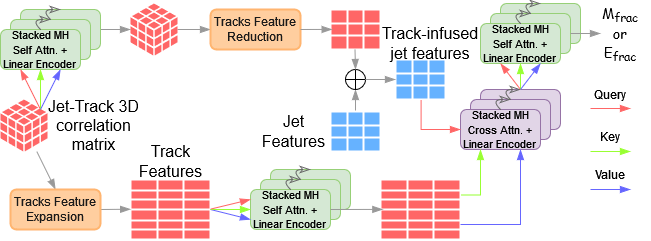
\includegraphics[width=1\linewidth]{PAKDD25-architecture.png}
\caption{Architecture of the proposed attention-based neural network method. Our method extracts two versions of track features to combine with jet features. The proposed multi-head cross-attention block correlates jets with respect to all tracks to enable learning of jet features based on an entire event.}
\label{fig:Model}
\end{figure}

%\rakib{We can say that here $\mathcal{J}$, $\emph{t}$ and $\mathcal{T}$ are jet features, track features independent of jets, and track features associated with jets, respectively.}


%as raw jet features: $[p_T,\eta,\phi,m]$, $\emph{t}$ as raw track features: $[p_T,\eta,\phi,m,d_0,z_0]$\footnote{Transverse, $d_0$, and longitudinal, $z_0$, distance to primary vertex when track is extrapolated to beam line using parameterized estimation}, and $\mathcal{T}$ as a 3d matrix which culminates the entire event with all jet and track features. Therefore, each event can be described by two tensors: a jet tensor $\mathcal{J}\in \mathbb{R}^{N_{J} \times F_{J}}$ and a track tensor $\mathcal{T} \in \mathbb{R}^{N_{J} \times N_{T} \times F_{T}}$ where $N_J$ is the number of jets in the event, $N_T$ is the number of tracks associated to $\mathbb{J}_i$, and $F_{J,T}$ is the number of features for jets and tracks, respectively. Therefore, the goal is to use the architecture in Figure \ref{fig:Model} to approximate the following function, $F(\mathcal{J},\mathcal{T}) \implies [Efrac,Mfrac]$, where Efrac and Mfrac have shape $N_{J}$. \\

% \begin{figure}[h]
% \centering
% \begin{subfigure}{1.0\textwidth}
% \centering
%   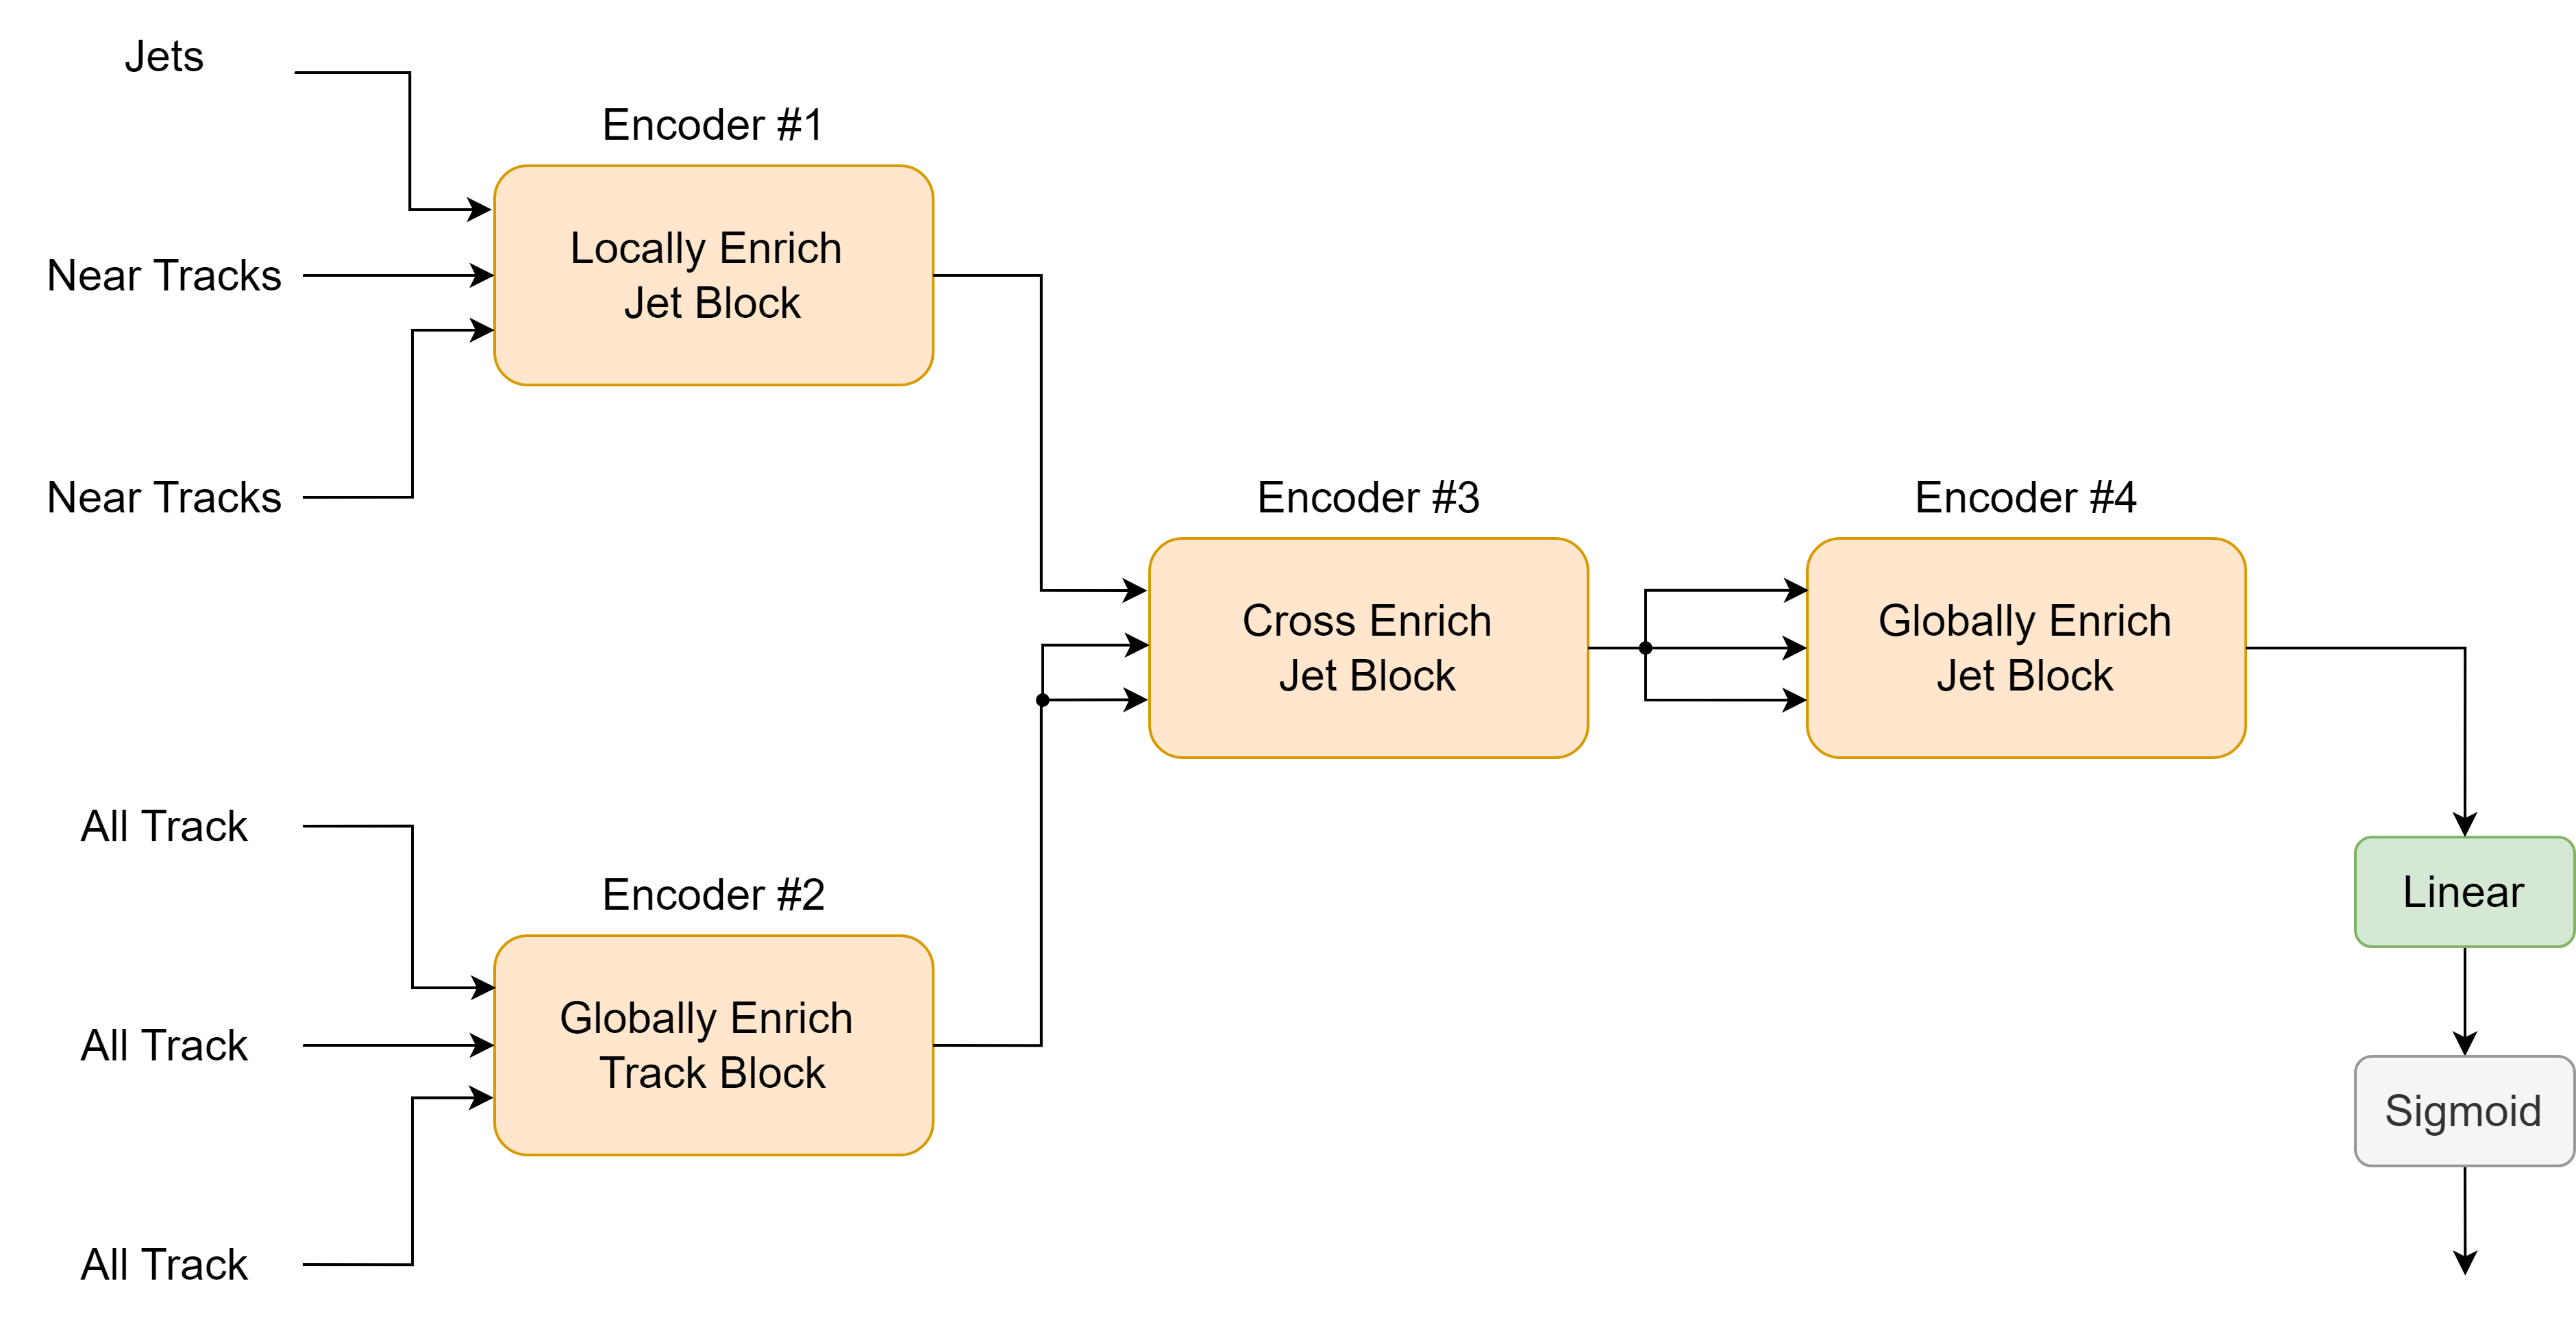
\includegraphics[width=0.70\linewidth]{figures/Physics-PileUp-v1.png}
%   \caption{}
%   \label{fig:sub1}
% \end{subfigure}%
% \hspace{-0.09cm}
% \begin{subfigure}{1.0\textwidth}
%   \centering
%   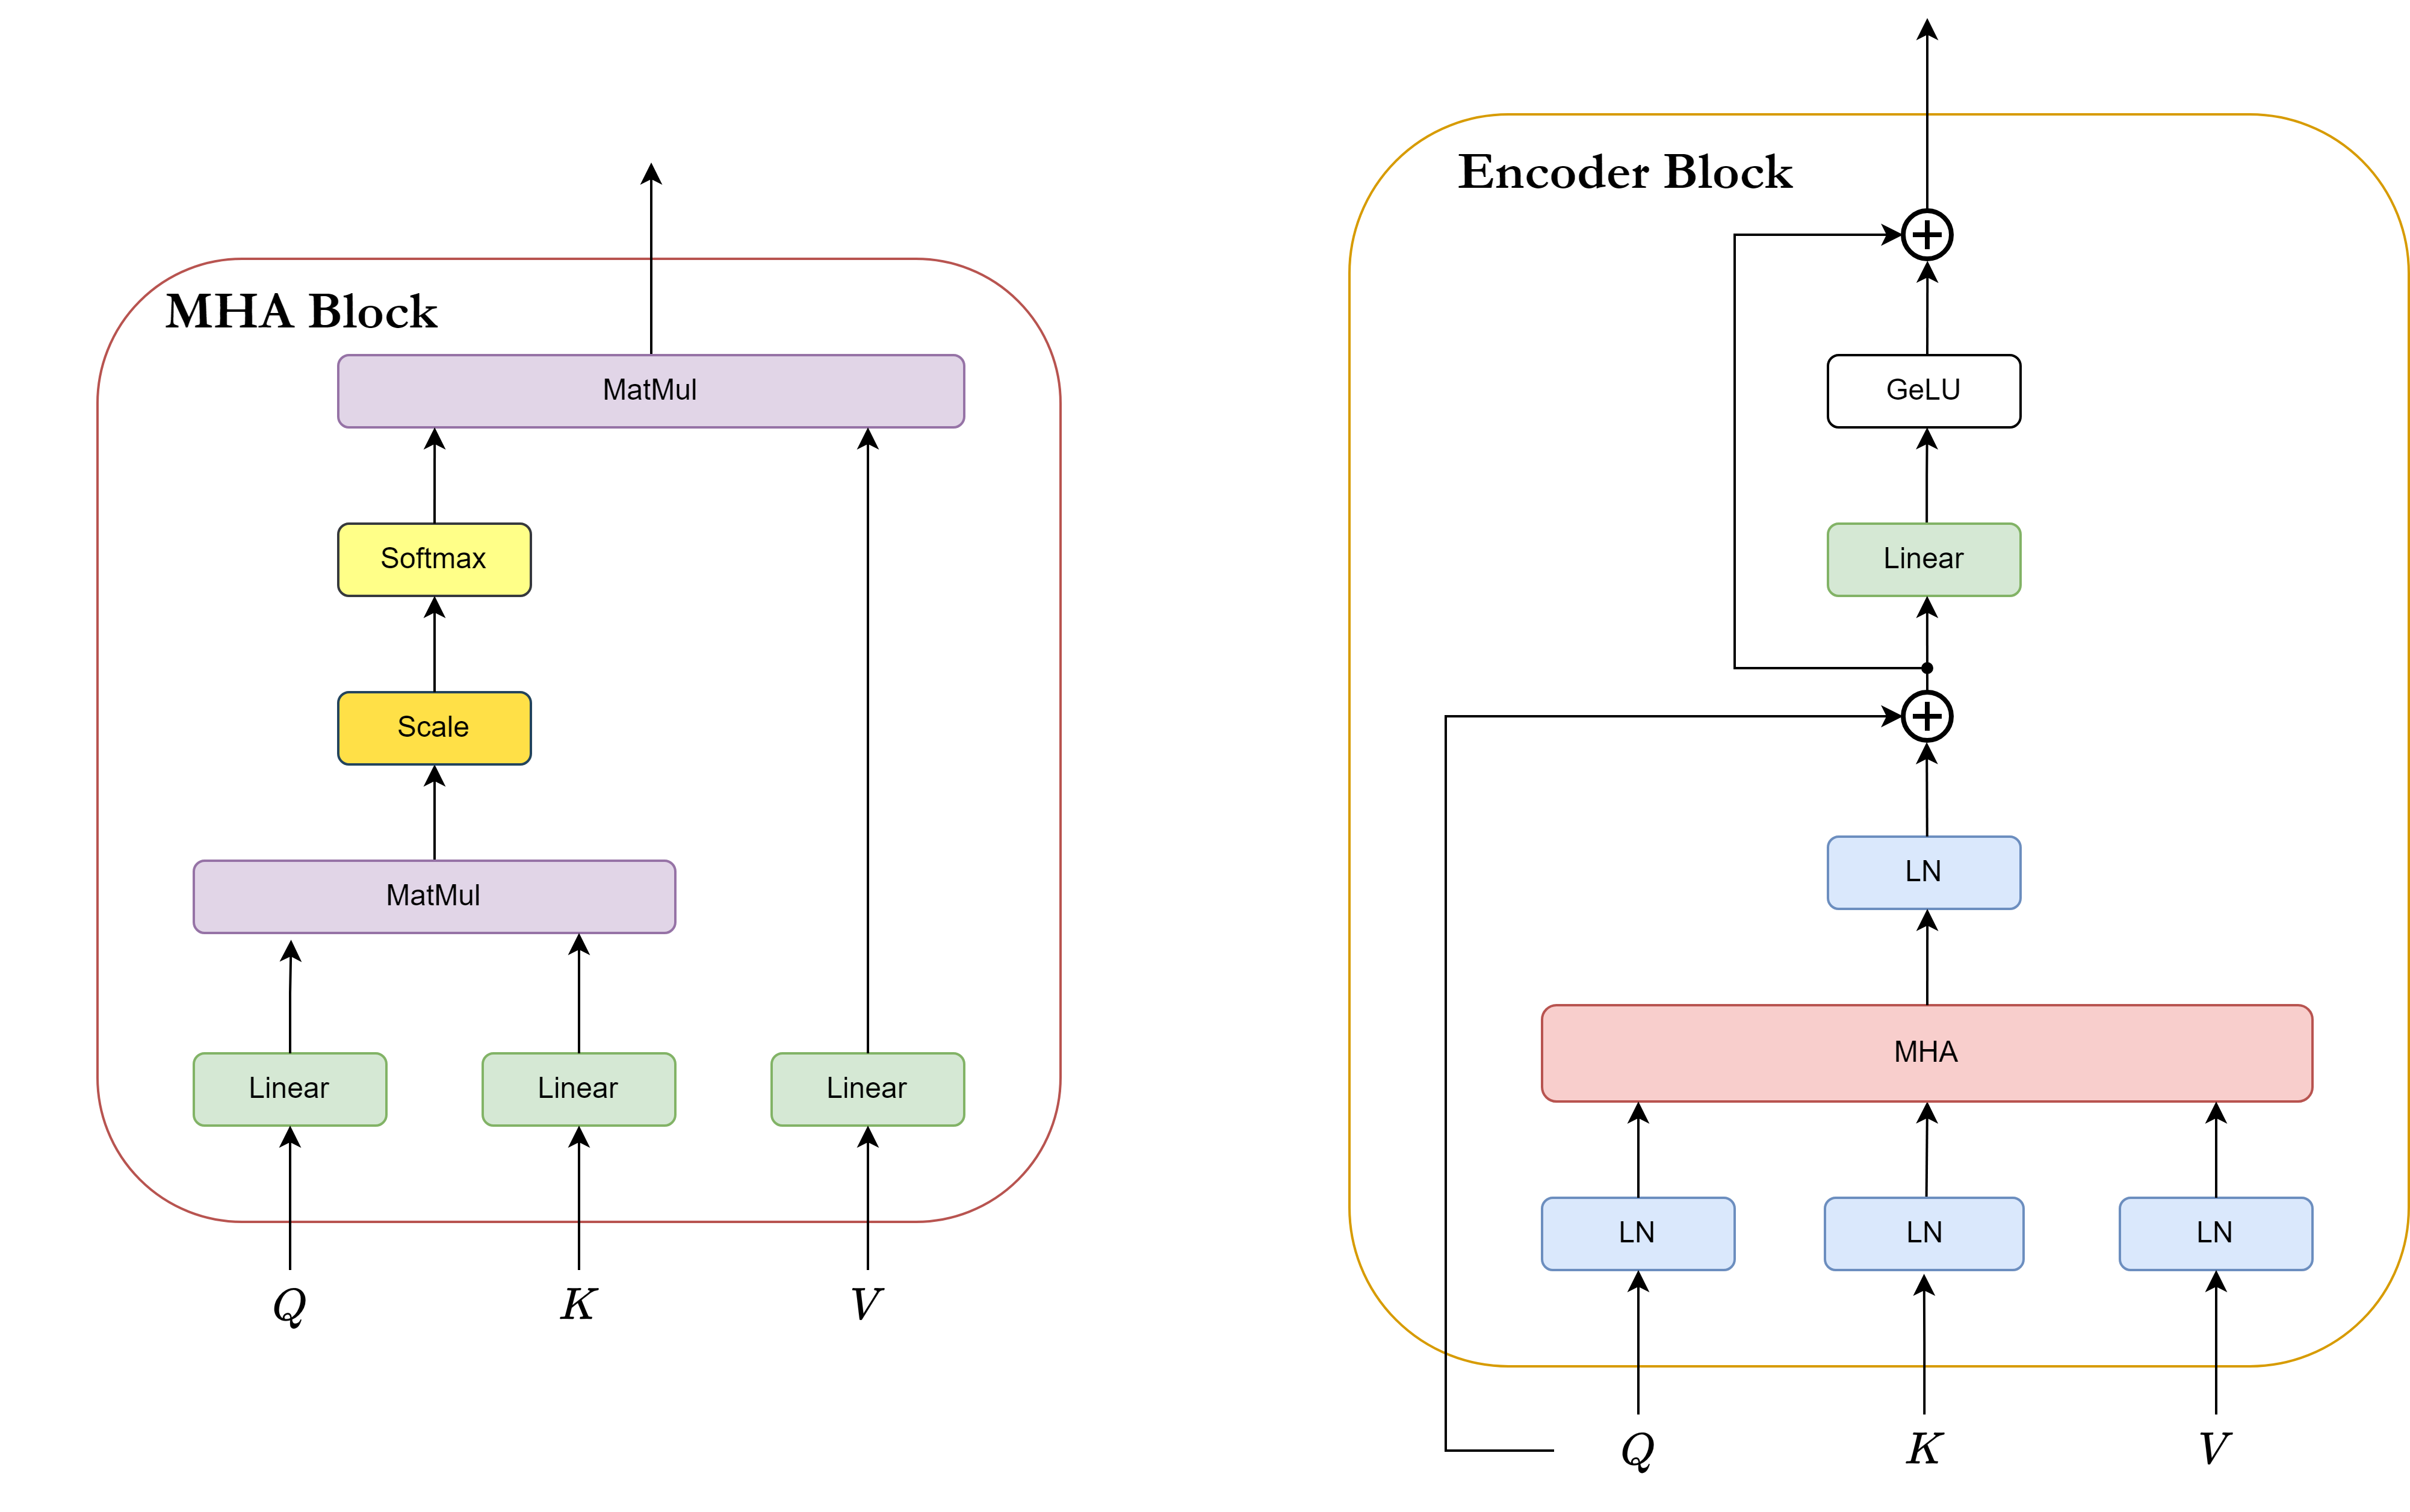
\includegraphics[width=0.70\linewidth]{figures/Physics-PileUp-Encoder-v1.png}
%   \caption{}
%   \label{fig:sub2}
% \end{subfigure}
% \caption{Beautiful Diagram of Model}
% \label{fig:Model}
% \end{figure}



\textbf{Transformer Encoders}: We incorporate encoders with two forms of Set Attention ~\cite{SetAttention} in this work: (i) \emph{Encoders with self-attention} to capture the dependencies of jets and tracks separately, and (ii) \emph{Encoder with cross-attention} to capture the dependencies between jets and tracks on each other. We employ the transformer encoder, which operates on inputs \(Q\) (query), \(K\) (key), and \(V\) (value). First, we apply scaled-dot product attention on normalized vectors to calculate the attention weights and extract correlations: $\text{Attention}(\mathbf{Q}, \mathbf{K}, \mathbf{V}) = \text{softmax}\left(\frac{\mathbf{Q} \mathbf{K}^\top}{\sqrt{d_E}}\right) \mathbf{V}$. We use multi-head attention, $MHA(Q,K,V) = $\\
$ Concat(Attention_1,\ldots,Attention_h)$, where $h$ is the total number of attention heads in the encoder. Second, a residual connections is used to generate the context vector: $\mathbf{Q}_\text{Context} = \mathbf{Q} + \text{MHA}(\mathbf{Q}, \mathbf{K}, \mathbf{V})$. Third, a feed-forward network and an additional skip connection are used to produce the updated representation of the input query: $\mathbf{Q}_\text{Output} = \mathbf{Q}_{\text{Context}} + \text{FFN}(\mathbf{Q}_{\text{Context}})$. This encoder block can be stacked numerous times to iteratively update the query with various key-value pairs. Therefore, the two types of encoders in \myname{} can be represented as given in Equation~\ref{eq:encoders} for inputs $\mathbb{X}$ and $\mathbb{Y}$:

\begin{equation}
    \text{Self-Encoder}(\mathbb{X},\mathbb{X},\mathbb{X}) = \mathbb{X}' \quad \text{Cross-Encoder}(\mathbb{X},\mathbb{Y},\mathbb{Y}) = \mathbb{X}'
    \label{eq:encoders}
\end{equation}

%We first use stacked self attention with linear encoders to learn high-dimensional features of $\emph{t}$ and $\mathcal{T}$.  In particular, we first apply linear transformations on these initial features using three weight parameters $W_q$, $W_k$, and $W_v$ to derive three distinct representations $Q$, $K$, and $V$, respectively, as given below. 

%Our approach leverages a transformer-based encoder to extract contextual representations of jets and tracks by capturing correlations within and between these inputs. The overall architecture of the model is shown in Figure~\ref{fig:Model}.

% \subsection{Transformer Encoder}

% The core building block of our model is a transformer encoder, which operates on inputs \(Q\) (query), \(K\) (key), and \(V\) (value). The encoder consists of the following components:

% 1. Layer Normalization: The inputs are normalized:
% \[
% \mathbf{Q} = \text{LN}(Q), \quad \mathbf{K} = \text{LN}(K), \quad \mathbf{V} = \text{LN}(V),
% \]
% where $\text{LN}(\cdot)$ denotes the layer normalization operation.

% 2. Self-Attention: Relationships between the inputs are computed using scaled dot-product attention:
% \[
% \text{Attention}(\mathbf{Q}, \mathbf{K}, \mathbf{V}) = \text{softmax}\left(\frac{\mathbf{Q} \mathbf{K}^\top}{\sqrt{d_E}}\right) \mathbf{V}.
% \]

% 3. Multi-Head Attention: Multi-head attention splits the embedding dimension \(d_E\) into \(h\) heads for parallel attention computation:
% \[
% \text{MHA}(\mathbf{Q}, \mathbf{K}, \mathbf{V}) = \text{Concat}(\text{head}_1, \ldots, \text{head}_h) \mathbf{W}_o,
% \]
% where $\text{head}_i = \text{Attention}(\mathbf{Q}_i, \mathbf{K}_i, \mathbf{V}_i)$, and $\mathbf{W}_o \in \mathbb{R}^{d_E \times d_E}$ is a learnable output projection matrix.

% 4. Residual Connection: The output of MHA is added back to the query:
% \[
% \text{Context} = \mathbf{Q} + \text{MHA}(\mathbf{Q}, \mathbf{K}, \mathbf{V}).
% \]

% 5. Feed-Forward Network (FFN): The context vector is refined through a feed-forward layer:
% \[
% \text{FFN}(\text{Context}) = \text{GELU}(\text{Context} \mathbf{W}_{\text{ff}} + \mathbf{b}_{\text{ff}}),
% \]
% where $\mathbf{W}_{\text{ff}} \in \mathbb{R}^{d_E \times d_E}$ and $\mathbf{b}_{\text{ff}} \in \mathbb{R}^{d_E}$ are learnable parameters. The final output of the encoder is:
% \[
% \text{Output} = \text{Context} + \text{FFN}(\text{Context}).
% \]

% This encoder is used iteratively in the following sections to process track, jet, and cross-attention features, adapting the query (\(Q\)), key (\(K\)), and value (\(V\)) inputs as per the task.


%\subsection{Feature Embedding}

\textbf{Learning Local Track-reinforced Jet Features $\hat{\mathcal{J}}$}: Apart from using jet features $\mathcal{J}$ for the underlying regression problems $f(\theta)$ and $g(\psi)$, transformer encoders can enrich a jet with its associated tracks for richer jet representations with respect to an event. To aggregate track features in jets, we first correlate jet and track features in the jet-track matrix $\mathcal{T}$ using $\mathcal{T}^{\prime} = \text{Self-Encoder}(\mathcal{T},\mathcal{T},\mathcal{T})$. We then aggregate tracks features of jets $\mathcal{J}_i$ using the sum operation, as given in Equation~\ref{eq:reduction}, where $N_T(\mathcal{J}_i)$ is the number of tracks in the jet $\mathcal{J}_i$. We then align the aggregated jet features $\hat{\mathcal{T}} \in \mathbb{R}^{N_J \times y}$ with the real jet features using the concatenation operation and apply non-linear transformation: $\hat{\mathcal{J}} = \text{ReLU}([\mathcal{J},\hat{\mathcal{T}}]W + b)$, where $W$ and $b$ are trainable weights and biases respectively.

\begin{equation}
\hat{\mathcal{T}}(\mathcal{J}_i) = \sum_{t=1}^{N_T(\mathcal{J}_i)} \mathcal{T}_{t}^{\prime}
\label{eq:reduction}
\end{equation}

\textbf{Learning Global Track Features $t$}: Apart from reinforcing jets with correlations based on local track features, we also aim to enrich jet features independently based on global track correlations during each event. To this end, we first flatten the jet-track correlation matrix $\mathcal{T}$ to consider only the track features $t \in \mathbb{R}^{N_{T} \ \times y}$, where $N_{T}$ is the total number of tracks in the event. We then enrich track features using the stacked self-encoder module: $\hat{t} = \text{Self-Encoder}(t,t,t)$. We emphasize that self-encoder modules on all tracks capture global contextual details in the event. 

\textbf{Learning Global Jet Features}: To model diverse event-wide correlations between jets $\hat{\mathcal{J}}$ and independent tracks $\hat{t}$, we apply encoder with cross-attention as $\mathcal{J}_{\text{cross}} = \text{Cross-Encoder}(\hat{\mathcal{J}},\hat{t},\hat{t})$. These encoded jet representations are based on the global context given by independent track representations that are present both within and outside the jets. Such unique representations allow the model to capture all possible correlations present in hard-scatter processes and give importance to learning jet features at the event-level. We further enrich these jet representations using $\mathcal{J}_{\text{final}} = \text{Self-Encoder}(\mathcal{J}_{\text{cross}},\mathcal{J}_{\text{cross}},\mathcal{J}_{\text{cross}})$.

% the transformer encoder is applied with:
% \[
% Q = \mathcal{J}_{\text{combined}}, \quad K = V = \emph{t}_{\text{embed}}.
% \]
% The output, \(\mathcal{J}_{\text{cross}}\), updates the jet embeddings based on the global context provided by the independent tracks:
% \[
% \mathcal{J}_{\text{cross}} = \text{Encoder}(\mathcal{J}_{\text{combined}}, \emph{t}_{\text{embed}}, \emph{t}_{\text{embed}}).
% \]

% The track aggregation (\ref{sec:trk-agg}) focuses on capturing fine-grained, local track-level details for each jet, while the cross-attention mechanism (\ref{sec:cross}) models global, event-level correlations between jets and independent tracks.

% The input features $\mathcal{J}$, $\emph{t}$, and $\mathcal{T}$ are first embedded into a high-dimensional space of size \(d_E\) using linear transformations followed by ReLU activation:
% \begin{align}
% \mathcal{J}_{\text{embed}} &= \text{ReLU}(\mathcal{J} \mathbf{W}_{\mathcal{J}} + \mathbf{b}_{\mathcal{J}}), \\
% \mathcal{T}_{\text{embed}} &= \text{ReLU}(\mathcal{T} \mathbf{W}_{\mathcal{T}} + \mathbf{b}_{\mathcal{T}}), \\
% \emph{t}_{\text{embed}} &= \text{ReLU}(\emph{t} \mathbf{W}_{\emph{t}} + \mathbf{b}_{\emph{t}}),
% \end{align}
% where $\mathbf{W}_{\mathcal{J}} \in \mathbb{R}^{x \times d_E}$, and \{$\mathbf{W}_{\mathcal{T}}$, $\mathbf{W}_{\emph{t}}$\} $\in$ $\mathbb{R}^{y \times d_E}$ are learnable weight matrices, and $\mathbf{b}_{\mathcal{J}}, \mathbf{b}_{\mathcal{T}}, \mathbf{b}_{\emph{t}} \in \mathbb{R}^{d_E}$ are learnable bias vectors. These embeddings form the initial representations used as inputs to the transformer encoder.


% \subsection{Track Aggregation}
% \label{sec:trk-agg}

% The transformer encoder is applied to the embedded track features (\(\mathcal{T}_{\text{embed}}\)) with:
% \[
% Q = K = V = \mathcal{T}_{\text{embed}}.
% \]
% The encoder output produces updated track embeddings:
% \[
% \mathcal{T}_{\text{updated}} = \text{Encoder}(\mathcal{T}_{\text{embed}}, \mathcal{T}_{\text{embed}}, \mathcal{T}_{\text{embed}}).
% \]
% These embeddings are aggregated across the track dimension for each jet:
% \[
% \hat{\mathcal{T}}_j = \sum_{t=1}^{N_T} \mathcal{T}_{\text{updated}, t}.
% \]

% \subsection{Jet Enrichment}

% The aggregated track embeddings \(\hat{\mathcal{T}}_j\) are concatenated with the jet embeddings \(\mathcal{J}_{\text{embed}}\) and passed through a linear layer followed by ReLU activation to refine the combined representation:
% \[
% \mathcal{J}_{\text{combined}} = \text{ReLU}([\mathcal{J}_{\text{embed}}, \hat{\mathcal{T}}_j] \mathbf{W}_{\text{post}} + \mathbf{b}_{\text{post}}),
% \]
% where \(\mathbf{W}_{\text{post}} \in \mathbb{R}^{2d_E \times d_E}\) and \(\mathbf{b}_{\text{post}} \in \mathbb{R}^{d_E}\). The resulting combined embeddings capture the local track information for each jet, enriched with both jet-level and track-level features.



% % \subsection{Cross-Attention Between Jets and Tracks}
% % \label{sec:cross}

% % To model event-wide correlations between jets and independent tracks (\(\emph{t}\)), the transformer encoder is applied with:
% % \[
% % Q = \mathcal{J}_{\text{combined}}, \quad K = V = \emph{t}_{\text{embed}}.
% % \]
% % The output, \(\mathcal{J}_{\text{cross}}\), updates the jet embeddings based on the global context provided by the independent tracks:
% % \[
% % \mathcal{J}_{\text{cross}} = \text{Encoder}(\mathcal{J}_{\text{combined}}, \emph{t}_{\text{embed}}, \emph{t}_{\text{embed}}).
% % \]

% % The track aggregation (\ref{sec:trk-agg}) focuses on capturing fine-grained, local track-level details for each jet, while the cross-attention mechanism (\ref{sec:cross}) models global, event-level correlations between jets and independent tracks.



% \subsection{Global Jet Contextualization}

% Finally, the enriched jet embeddings \(\mathcal{J}_{\text{cross}}\) are refined using self-attention across all jets:
% \[
% Q = K = V = \mathcal{J}_{\text{cross}}.
% \]
% The encoder output produces the final jet embeddings:
% \[
% \mathcal{J}_{\text{final}} = \text{Encoder}(\mathcal{J}_{\text{cross}}, \mathcal{J}_{\text{cross}}, \mathcal{J}_{\text{cross}}).
% \]

\textbf{Learning Objective}: We predict $E_{frac}$ and $M_{frac}$ using final jet features \(\mathcal{J}_{\text{final}}\) by attaching the regression layer with sigmoid activation function ($\sigma$): $\hat{y} = \sigma(\mathcal{J}_{\text{final}} \mathbf{W}_{\text{out}} + \mathbf{b}_{\text{out}})$, where $\mathbf{W}_{\text{out}}$ and $\mathbf{b}_{\text{out}})$ are learnable regression weights and biases. We optimize all model parameters to learn optimal jet and track features in a supervised fashion using the Mean Squared Error loss function:
\[
\mathcal{L} = \frac{1}{N} \sum_{i=1}^N \left( \hat{y}_i - y_i \right)^2,
\]
where \(N\) is the total number of training samples, $y$ is the ground truth ($E_{frac}$ or $M_{frac}$), and $\hat{y}$ is the model prediction. By leveraging track features and global context through iterative encoder-based attention mechanisms, the model progressively refines jet features to predict energy and mass fractions with least mean square error.


% \subsection{Regression}

% The final jet embeddings, \(\mathcal{J}_{\text{final}}\), are passed through a regression layer with sigmoid activation to predict \(E_{\text{frac}}\) and \(M_{\text{frac}} \):
% \[
% \hat{y} = \sigma(\mathcal{J}_{\text{final}} \mathbf{W}_{\text{out}} + \mathbf{b}_{\text{out}}),
% \]
% where \(\mathbf{W}_{\text{out}} \in \mathbb{R}^{d_E \times 1}\) and \(\mathbf{b}_{\text{out}} \in \mathbb{R}\). This layer maps the enriched jet embeddings to the desired output space, producing predictions for the energy and mass fractions.

% \subsection{Learning Objective}

% The model is trained using the mean squared error (MSE) loss, which minimizes the difference between the predicted values, \(\hat{y}\), and the ground truth labels, \(y\):
% \[
% \mathcal{L} = \frac{1}{N} \sum_{i=1}^N \left( \hat{y}_i - y_i \right)^2,
% \]
% where \(N\) is the total number of training samples.

% By leveraging track features and global context through iterative encoder-based attention mechanisms, the model progressively refines jet embeddings to predict energy and mass fractions with high accuracy.


% We use multihead self attention~\cite{Attention} to learn attention weights of tracks and jet-tracks which are then combined with values to derive contextual representations. We further use linear layer and a feed forward neural network to obtain , as given in the following equations, which captures inherent semantically important information present within $\emph{t}$ correlations and $\mathcal{T}$ correlations respectively.  

% \arun{multihead and NN equations go here}

%overall model architecture can be considered a stack of various transformer encoders using multi-head attention~\cite{Attention} to approximate the optimal high-dimensional embedding of jets in the context of an event. Since a jet itself is only described by four features, various transformer encoders use self attention to capture track-track and jet-jet correlations and cross attention to capture jet-track correlations which heavily enriches the embedded representation of a jet. 

% Effectively, apart from using jet features for the underlying regression problems $f(\theta)$ and $g(\psi)$, transformer encoders can enrich a jet with its associated tracks and all other possible information from the event allowing for a richer embedded representation. It is with these enriched jet embeddings that the model is able to learn, from data, the hard scatter energy and mass fractions of each jet in an event.

% \begin{equation}
%     \hat{\mathcal{T}}_j = \sum_{t=1}^{|\mathcal{T}_J|} \mathcal{T}_{jt}
% \end{equation}

% In real-world experiments, jet features can be largely aligned with tracks associated with them. We combine jet features with track features that are reduced from jet-track features using a linear operation such as concatenation: $\mathcal{J} = \mathcal{J} \oplus \hat{\mathcal{T}}$.

% With context enriched jet features and track features, it is necessary to understand correlations of jets, not only with tracks within, but also with tracks outside them. We employ cross-encoder module, as given in Equation , to learn these diverse correlations between jets and tracks. This cross encoder module allows jets to update their representations with tracks outside their cone, which allows the model to capture all possible correlations present in hard-scatter processes.

% \arun{Cross attention block goes here}

% \arun{Learning objective}

%\luke{vvvvvv  This paragraph is bad but I am trying to explain the encoders}\\
%Each encoder block uses a Query and Key-Value pair to enrich a set of queries in the context of a set of keys. Due to the inherent unordered nature of sets, no position encoding is required. Scaled dot product attention is used to generate attention weights, an $N \times M$ matrix, where $N$ and $M$ are the cardinality of the query and key sets, respectively. These attention weights allow the model to learn correlations between elements of the query and key set which is fundamentally required to extract the hard scatter correlations present in the dataset. Layer normalizations are used to stabilize the training process REF [NORMFORMER]. The output of the MHA block can be interpreted as a \emph{context} vector that can be added element wise to the query through a skip connection. This combined vector is passed through a linear layer with GeLU activation and another skip connection is applied to deliver the updated representation of the query set in the context of the key set. \\

% Tensors $\mathcal{J}$ and $\mathcal{T}$ are first processed using linear layer with GeLU activation to transform from the feature space to an initial embedding space, $F_{J,T} \rightarrow d_E$. Then two types of encoders are used:
% \begin{equation}
%   \text{Self-Encoder}(\mathbb{X},\mathbb{X},\mathbb{X})=\mathbb{X}' \phantom{.......} \text{Cross-Encoder}(\mathbb{X},\mathbb{Y},\mathbb{Y})=\mathbb{X}'
% \end{equation}
%where $\mathbb{X}$ and $\mathbb{Y}$ are sets representing Query, Key, and Value. First, jets are enriched using their associated tracks using the "Locally Enrich Jet Encoder Block". 

% This is done by: $\text{Self-Encoder}(\mathcal{T},\mathcal{T},\mathcal{T})=\mathcal{T}'$, reduction operation over $N_T$ dimension, then concatenated with the $\mathcal{J}$ tensor along $d_E$ dimension to form tensor $\mathcal{J}'$. Second, tracks are enriched at the event level by flattening along $N_T$ dimension to form $\mathcal{T}_{flat}$, and passed through "Globally Enrich Track Block", $\text{Self-Encoder}(\mathcal{T}_{flat},\mathcal{T}_{flat},\mathcal{T}_{flat})=\mathcal{T}_{flat}'$. This block allows hard scatter tracks to pass information throughout the entire event. Third, the novel "Cross Enrich Jet Block" uses $\text{Cross-Encoder}(\mathcal{J}',\mathcal{T}_{flat}',\mathcal{T}_{flat}')=\mathcal{J}''$. This cross encoder block allows jets to update their representations with tracks outside their cone, which allows the model to capture all possible correlations present in hard scatter processes. Fourth and finally, the "Globally Enrich Jet Encoder Block" is used to update jets in the context of an entire event, $\text{Self-Encoder}(\mathcal{J}'',\mathcal{J}'',\mathcal{J}'')=\mathcal{J}_{Event}$. This tensor, $\mathcal{J}_{Event}$, represents the high dimensional embeddings of the jets in the event, and can be used to quantify the amount of pileup, Efrac and Mfrac, using a final regression layer with sigmoid activation. \\

% The model is trained on the diHiggs simulated dataset, described in Section \ref{Dataset} depicted in Figure \ref{fig:HLLHC}, using Efrac and Mfrac as targets, described in Section \ref{JetLabels} depicted in Figure \ref{fig:Labels}. In practice, each encoder block is duplicated 3 times to give the model more learnable parameters, $\sim$4.1M,  to achieve a deeper representation of jets. During the training process, the learning rate is scheduled to decay by a factor of 0.1 after the 25th epoch which noticeably helped descend the noisy loss landscape. The AdamW optimizer is used to prevent overtraining using weight decay, and Mean Squared Error was used as the loss function. The model converged after training 50 epochs on an NVIDIA RTX 3090.


%The model is trained on the diHiggs simulated dataset, described in Section \ref{Dataset} depicted in Figure \ref{fig:HLLHC}, using Efrac and Mfrac as targets, described in Section \ref{JetLabels} depicted in Figure \ref{fig:Labels} using a Mean Squared Error loss function.



%%%%%%%%%%%%%%%%%%%%%%%%%%
%%% Multi-Line Comment %%%
%%%%%%%%%%%%%%%%%%%%%%%%%%
\iffalse
\subsection{Model Architecture}\hfill

Four transformer encoder stacks are used to enrich each tensor -- $\mathbb{J},\mathbb{T}_{jet},\mathbb{T}_{jet}$ -- with context from the event. Each encoder follows the NormFormer [*] architecture by (... et al). NormFormers consists of LayerNorms, LN(), multi-head attention, MHA(), skip connections, + operator, feed-forward network, FFN, which consists of a linear layer and a GELU activation function. These layers are the components of each encoder block.


First, each jet is enriched with associated tracks. Since each jet only carries four features, $p_T, \eta, \phi, m$, tracks within a radius of $\Delta R = 0.4$ are used in the first encoder stack to achieve a rich representation of each jet.

\begin{align}
    \mathbb{T}_{context} &= \mathbb{T}_{jet} + LN(MHA(LN(\mathbb{T}_{jet}), LN(\mathbb{T}_{jet}), LN(\mathbb{T}_{jet}))) \\
    \mathbb{T}_{embed} &= \mathbb{T}_{context} + FFN (\mathbb{T}_{context}) \\
    \mathbb{T}_{aggregated} &= \sum_{dim=1} \mathbb{T}_{embed} \\ 
    \mathbb{J}_{enriched} &= FFN(\mathbb{J} \mathop{\oplus}_{dim=1} \mathbb{T}_{aggregated})
\end{align}
$\mathbb{T}_{jet}$, $\mathbb{T}_{context}$, and $\mathbb{T}_{embed}$ all have shape $N_{jet} \times N_{trk} \times E_{dim}$. Then the summation operator reduces the $N_{trk}$ dimension which will then match the dimension of $\mathbb{J}$ with shape $N_{jet} \times E_{dim}$. The jet and aggregated track tensors are concatenated along the embedding dimension, and the FFN has input $N_{jet} \times 2\cdot E_{dim}$ and outputs $\mathbb{J}$ of shape $N_{jet} \times E_{dim}$. This encoder block can be interpreted physically as learning to enrich the jet in the context of associated particles. %For example, if there is are particles that resemble b-hadron decay, this encoder block might enrich this jet as a b-jet in the latent space.

Second, $\mathbb{T}_{event}$ with shape $N_{trk} \times E_{dim}$ are enriched using an encoder block using self-attention:
\begin{align}
    \mathbb{T}_{context} &= \mathbb{T}_{event} + LN(MHA(LN(\mathbb{T}_{event}), LN(\mathbb{T}_{event}), LN(\mathbb{T}_{event}))) \\
    \mathbb{T}_{embed} &= \mathbb{T}_{context} + FFN (\mathbb{T}_{context})
\end{align}
The purpose of this encoder is to update all tracks in the context of the event and initialize them for cross attention with jets.

Third, cross attention between $\mathbb{J}_{enriched}$ and $\mathbb{T}_{embed}$ is performed to update the jets in the context of all tracks of the event.

\begin{align}
    \mathbb{J}_{context} &= \mathbb{J}_{enriched} + LN(MHA(LN(\mathbb{J}_{enriched}), LN(\mathbb{T}_{event}), LN(\mathbb{T}_{event}))) \\
    \mathbb{J}_{embed} &= \mathbb{J}_{context} + FFN (\mathbb{J}_{context})
\end{align}

%This encoder allows tracks to update the jet embedding in the context of an event. For example, if we consier $t \rightarrow Wb \rightarrow l\nu b$, this encoder allows the high energy lepton, l, to update the context of the b-jet.

Fourth and finally, $\mathbb{J}_{embed}$ with shape $N_{jet} \times E_{dim}$ is enriched using a encoder block using self attention:

\begin{align}
    \mathbb{J}_{context} &= \mathbb{J}_{embed} + LN(MHA(LN(\mathbb{J}_{embed}), LN(\mathbb{J}_{embed}), LN(\mathbb{J}_{embed}))) \\
    \mathbb{J}_{embed} &= \mathbb{J}_{context} + FFN (\mathbb{J}_{context})
\end{align}

This encoder is performed last because at this stage the jets have achieved a rich representation after passing through the previous encoders. This last encoder allows jets to update their representation in the context of an event. This encoder can be interpreted physically as allowing jets to update representations according to conservation of momentum or other properties that might be shared between jets.

Lastly, the embedded jet vectors are passed through a final classification layer to predict the continuous Efrac and Mfrac label.
\fi
%%%%%%%%%%%%%%%%%%%%%%%%%%
%%% Multi-Line Comment %%%
%%%%%%%%%%%%%%%%%%%%%%%%%%
